\documentclass[a4paper, 12pt]{article}

\usepackage{listings}
\usepackage{indentfirst}
\usepackage{graphicx}
\usepackage{pdfpages}

\usepackage{color}

\definecolor{mygreen}{rgb}{0,0.6,0}
\definecolor{mygray}{rgb}{0.5,0.5,0.5}
\definecolor{mymauve}{rgb}{0.58,0,0.82}

\lstset{ 
  backgroundcolor=\color{white},   % choose the background color; you must add \usepackage{color} or \usepackage{xcolor}; should come as last argument
  basicstyle=\footnotesize,        % the size of the fonts that are used for the code
  breakatwhitespace=false,         % sets if automatic breaks should only happen at whitespace
  breaklines=true,                 % sets automatic line breaking
  captionpos=b,                    % sets the caption-position to bottom
  commentstyle=\color{mygreen},    % comment style
  deletekeywords={...},            % if you want to delete keywords from the given language
  escapeinside={\%*}{*)},          % if you want to add LaTeX within your code
  extendedchars=true,              % lets you use non-ASCII characters; for 8-bits encodings only, does not work with UTF-8
  keepspaces=true,                 % keeps spaces in text, useful for keeping indentation of code (possibly needs columns=flexible)
  keywordstyle=\color{blue},       % keyword style
  language=Octave,                 % the language of the code
  morekeywords={*,...},            % if you want to add more keywords to the set
  numbers=left,                    % where to put the line-numbers; possible values are (none, left, right)
  numbersep=5pt,                   % how far the line-numbers are from the code
  numberstyle=\tiny\color{mygray}, % the style that is used for the line-numbers
  rulecolor=\color{black},         % if not set, the frame-color may be changed on line-breaks within not-black text (e.g. comments (green here))
  showspaces=false,                % show spaces everywhere adding particular underscores; it overrides 'showstringspaces'
  showstringspaces=false,          % underline spaces within strings only
  showtabs=false,                  % show tabs within strings adding particular underscores
  stepnumber=2,                    % the step between two line-numbers. If it's 1, each line will be numbered
  stringstyle=\color{mymauve},     % string literal style
  tabsize=2,	                   % sets default tabsize to 2 spaces
  title=\lstname                   % show the filename of files included with \lstinputlisting; also try caption instead of title
}

%===========================================%
%=               Credits                   =%

\author{Name}
\title{Title}

%=                                         =%
%===========================================%

%===========================================%
%=               BEGIN                     =%

\begin{document}
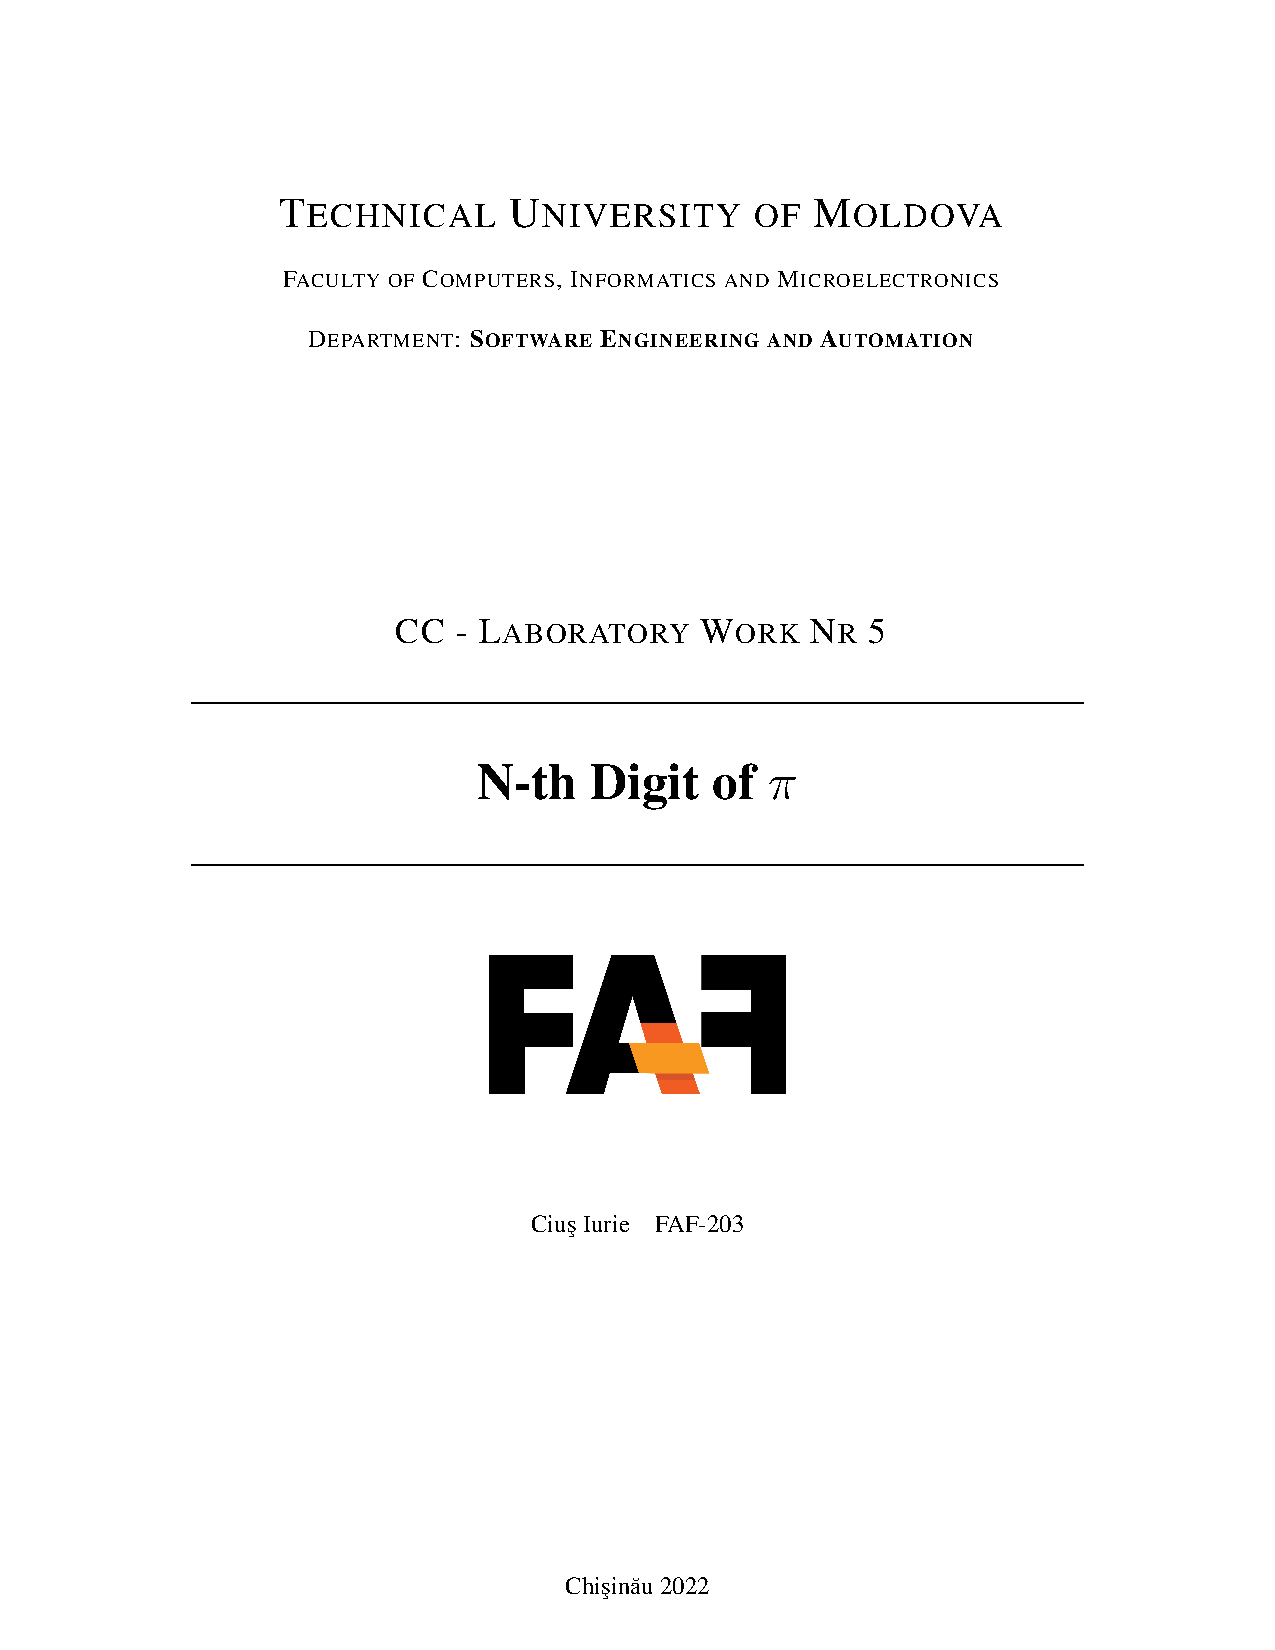
\includepdf[pages={1}]{title.pdf}
\tableofcontents
\newpage

\section{Algorithm Analysis}

Algorithm analysis is an important part of computational complexity theory, which provides
theoretical estimation for the required resources of an algorithm to solve a specific computational problem. Analysis of algorithms is the determination of the amount of time and space
resources required to execute it.

\subsection{Introduction}

The current paper work represents my implementation of two algorithms to determine the N-th digit of $\pi$.
The fascination of the number $\pi$ by mathematicians is ancient, and numerous computations of its
digits have been performed in the history. Later, computers have been used to increase the number
of computed digits
There are multiple ways by which we can calculate the nth digit of pi by using \textbf{Arctan formula} and \textbf{Bailey–Borwein–Plouffe formula.
    Chudnovsky Algorithm} is a fast way of calculating the digits of pi and is similar to the arctan's formula.

$$
    \pi + 3 = \sum_{k>0} \frac{k2^k}{(\frac{2k}{k})}
$$

This formula has no big powers of primes in denominators, and this was the key success factor in
\textbf{Plouffe} approach.

Later, based on the same formula, Fabrice Bellard refined Plouffe technique with
an algorithm using $O(n^2)$ elementary operations on numbers of size $O(logn)$.

\newpage

\subsection{Objectives}

\begin{itemize}
    \item Implement at least 2 algorithms to determine the N-th digit of $\pi$.
    \item Establish the properties of the input data in relation to which the analysis is made.
    \item Choose the metric for comparing algorithms.
    \item Perform empirical analysis of the proposed algorithms.
    \item Make a conclusion on the work done.
\end{itemize}

\subsection{Theoretical Notes}

Our starting point is the classical following alternating series to compute $\pi$:

\[ \frac{\pi}{4} = arctan(1) = \sum_{k=0}^{\infty}\frac{(-1)^k}{2k+1} \]

In this form, the formula is well suited to nth decimal digit computation, but its convergence
is too slow.

Let an alternating series of the form:

\[ S = \sum_{k=0}^{\infty} (-1)^k a_k \]

where we assume that there exists a positive function weight $w(x)$ such that

\[ a_k = \int_0^1 x^k w(x) dx. \]

Various acceleration convergence techniques exist for such series (finite differences Euler acceleration process for example, ...), and can be generalized with the following result from Cohen,
Villegas and Zagier.

Let $ P_n(x) = \sum_{k=0}^n p_k(-x)^k $  a degree n polynomial for which $ P_n(-1) \neq 0 $. We define:

\[ |S_n-S| <= \frac{1}{|P_n(-1)|}\int_0^1 \frac{|P_n(x)|w(x)}{1+x} dx \leq \frac{M_n}{|P_n(-1)|}S \]

\newpage

\subsection{Description of the algorithm}

\textbf{Algorithm 1 (n-th digit computation of $\pi$ with very low memory)} \textit{The following algorithm
    computes the fractional part of $10^n\pi$ with an error $< 10^{-n_0}$ when $n \geq 4n_0$.}

$$$$

\textit{1. Define integers M and N by}

$$
    M = 2 \left[\frac{n}{log^3(n)}\right] \quad and \quad N = \left[(n+n_0+1)\frac{log(10)}{log(2eM)}\right]
$$

\textit{2. (Computation of B) Initialize b = 0 a floating point value. For index k, $0 \leq k < (M + 1)N$ perform the following operations :}

\begin{itemize}
    \item Compute $x = 4 \times 10^n \ mod \ 2k+1$
    \item Compute $b := \{b+(-1)^kx/(2k+1)\}$
\end{itemize}

\textit{3. (Computation of C) Initialize c = 0 a floating point value. For index $k, 0 \leq k < N$ perform
    the following operations}

\begin{itemize}
    \item Compute $x = \sum_{j=0}^k (N j) mod (2MN + 2k + 1)$
\end{itemize}

\textit{4. (Final step) Compute the value x as the fractional part of $b - c (x = b - c - [b - c])$. Then
x is an approximation of $\{10n\pi\}$ with an error less than $10-n_0$.
}

\newpage

\section{Code}

The following chapter represents my implementation and results of the current laboratory work.

\subsection{Implementation}

\lstinputlisting[language=Python]{script.py}
\lstinputlisting[language=Java]{script.js}
\subsection{Complexity of the algorithm}

\textbf{Lemma 1} \textit{For $k < N < m$, algorithm 2 has a memory need of $O(log^2m)$ bits and time complexity of}

$$
    Cost_2(m) = O(log(m)) + O(k) + O(\lambda_k(m)k)
$$

\textit{elementary operations on numbers of size $O(log(m))$, where $\lambda_k(m)$ is the number of distinct prime factors p of m such that $p \leq k$.}

\subsection{Graphs}

\begin{center}
    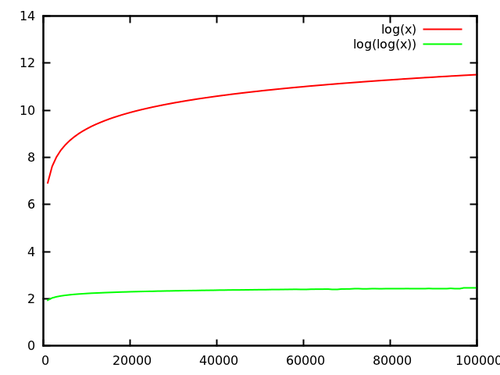
\includegraphics[width=15cm]{graph.png}
\end{center}

\section{Conclusion}

During this laboratory work, I studied and analyzed two
of the most popular algorithms to find the n-th digit of $\pi$, each with it's upsides and downsides.

On the one hand, we have been able to obtain an algorithm to compute directly the n-th decimal
digit of $\pi$ in nearly quadratic time and using only O(log2
n) memory; on the other hand, computing
all the first n digits of $\pi$ is possible in quasi-linear time and with memory O(n).
\subsection{References}

\begin{itemize}
    \item https://github.com/IuraCPersonal/FAF203-CC
\end{itemize}

\end{document}